\documentclass{beamer}

% \usepackage{beamerthemesplit} // Activate for custom appearance

\usepackage{graphicx}


\title{{\small INFO 411 presentation on:} \\ \bigskip Callaghan et
  al. (2002) {\em Streaming-Data Algorithms for High-Quality
    Clustering}} \author{Noel Park, Kat Lilly and Loren Kersey}
\date{\today}

\begin{document}

\frame{\titlepage}

\section[Outline]{}
\frame{\tableofcontents}

\section{Introduction, Background}

\frame
{
  \frametitle{Introduction - Datasets vs Data streams}

  Datasets
  \begin{itemize}
    \item Large volume of stored data (static).
    \item Appropriate for querying model based on unchanging data.
    \item Concept drift.
    \newline
  \end{itemize}

  Data stream:
  \begin{itemize}
    \item Large volume continuously arriving data (dynamic).
    \item Unnecessary, or impractical to store data in memory.
  \end{itemize}
}

\frame
{
  \frametitle{Introduction - Data stream model}

  Data stream models are mainly restricted by:
  \begin{itemize}
    \item process data sequential (no random access).
    \item small memory consumption (limited storage).
    \newline
  \end{itemize}

  The Challenge is to perform meaningful computations within these restrictions. \newline

  This paper by O'Callaghan et al. (2002) describes a streaming
  algorthim that effectively clusters large data streams.

  %NOTES: 
  % item 3: random access to memory not allowed.
  % item 4: limited amount of information can be stored.
  % challenge is to perform meaningful computations within these restrictions.
}

\frame
{
  \frametitle{Application Example - Intrusion Detection}
  
  They were able to demonstrate network intrusion detection. \newline

  Dataset:
  \begin{itemize}
    \item KDD-CUP99 dataset (743 MB, simulates intrusion in military networks)
    \item Dataset contains raw TCP dump data.
    \item Contains 42 attributes like TCP connection duration, failed login attempts, etc.
    \newline
  \end{itemize}
}

\frame
{
  \frametitle{Application Example - Intrusion Detection}

  They were able to demonstrate network intrusion detection. \newline

  Simulation:
  \begin{itemize}
    \item Simulated network stream by processing dataset in 16MB chunks.
    \item Their algorithm clustered data into 5 clusters (4 types of attacks and no attack).
    \item DDOS, password guessing, unauthorized access to root, probing (port scanning). 
  \end{itemize}
}

\section{The new algorithm described in this paper}

\frame
{
  \frametitle{The Clustering Problem}

  The problem this paper focuses on is the following version of the
  clustering problem: 
  
  \begin{itemize}
  \item given an integer {\em k} and a dataset {\em N}, find {\em k}
    cluster centers and assign each {\em n} to the nearest centre
  \item measure the quality of the clustering by the sum of the
    squared distances (SSQ) of the data points to their assigned centers.
  \item Find an optimal or near optimal solution by minimising SSQ.
  \end{itemize}

  The general K-median problem is an NP-hard problem, but there are
  various algorithms for SSQ minimisation that produce near-optimal
  solutions in near-linear time.

  \bigskip
  This paper describes a new such algorithm suitable for streaming
  data.
  
}

\frame
    {
      \frametitle{Facility Location Problem}

      One benefit of the algorithm described in this paper is that it is
      flexible in the value of {\em k}.
      \begin{itemize}
      \item Instead of specifying a limit on the value of {\em k}, impose
        a cost for each cluster center (called a `facility' here).
      \end{itemize}

      \bigskip
      The aim now is to minimise the sum of both the distance metrics and
      the facility costs,
      \begin{itemize}
      \item so long as a suitable value for the facility cost is
        chosen, an appropriate number of clusters will be found.
      \end{itemize}

      \bigskip
      Again this is an NP-hard problem, but several algorithms are
      known that produce near-optimal solutions.
      
    }

\frame
    {
      \frametitle{Finding an appropriate facility cost}

      Their solution is to set an upper and lower bound on the value of {\em z},
      the facility cost, and perform a binary search within this range to
      find a suitable value
      \begin{itemize}
      \item Lower bound: 0
      \item Upper bound: calculated from the sum of the distances
      \end{itemize}

      \bigskip
      At each {\em z} value in this search they calculate a solution
      \begin{itemize}
      \item if that solution has the desired number of clusters they
        have found a suitable {\em z} value
      \end{itemize}
      They then use this {\em z} value to find the best value for {\em k}.

      \bigskip
      Their solution is guaranteed to find the facility cost that will
      result in the correct value for {\em k} in a dataset that is
      `naturally k-clusterable'.

      
    }


\frame
{
  \frametitle{STREAM Algorithm}

  They call the new algorithm described in this paper `STREAM'.

  \bigskip
  Data is clustered in small chunks - either the data
  arrives this way or they wait until enough data arrives to deal with
  it this way.

  \bigskip
  Each chunk of data in the stream is clustered with their new
  algorithm `LSEARCH'.

}



\frame
{
  \frametitle{STREAM algorithm}


 Once the clustering of each chunk is done, the original data is
 discarded, and only the {\em k} cluster centers are stored. Each
 cluster being weighted by the sum of the weights of its members.

 \bigskip
 The number of points stored in memory at any given time is {\em ik},
 where {\em i} is the number of chunks of data processed and {\em k}
 is the number of clusters.

 \bigskip
 If the number of points in memory becomes too large, at any point we
 can cluster the {\em ik} clusters to reduce the data to just {\em k}
 clusters.

}


\frame
    {
      \frametitle{LSEARCH algorithm}
      \begin{enumerate}
      \item Find a value for the facility cost that results in desired k
        \begin{itemize}
        \item {\bf inputs:} dataset, z-min, z-max
        \item {\bf ouput:} k
        \end{itemize}

      \item Find an initial solution
        \begin{itemize}
        \item {\bf inputs:} dataset, z
        \item {\bf output:} a solution, consisting of a list of
          centres and an assignment function
        \end{itemize}
        
      \item Facility location
        \begin{itemize}
        \item {\bf inputs:} dataset, distance metric, z, epsilon, initial solution (centres
        and assignment function)
        \item {\bf ouput:} a set of facilities (clusters centres) and a function
          that assigns datapoints to clusters.
        \end{itemize}
   \end{enumerate}
    }


\section{Comparison with existing methods}
\frame
{
  \frametitle{Comparison with other methods}
  To assess the performance of their new clustering and streaming algorithms, O'Callaghan et al. compare them to existing techniques.
  
  \bigskip 
  \begin{itemize}
  \item{LSEARCH performs a similar function to k-means}
  \item{STREAM performs a similar function to BIRCH
    \begin{itemize}
      \item{BIRCH - balanced iterative reducing and clustering using hierarchies - is another streaming algorithm which uses a clustering algorithm as a sub-routine.}
    \end{itemize}
  }
  	     
  \end{itemize}
}

\frame
{
  \frametitle{LSEARCH vs k-means}
  
  \begin{columns}
  
    \begin{column}{0.5\textwidth}
       \begin{itemize}
          \item{Generated 28 small data-sets with between 5 and 16 uniform density spheres}
          \item{For each data-set, calculate SSQ to use as an upper-bound for the optimal SSQ}
          \item{Overlay each data-set with random noise}
          \item{Run LSEARCH and k-means 10 times over each data-set}
      \end{itemize}
    \end{column}
    
    \begin{column}{0.5\textwidth}
        \begin{center}
         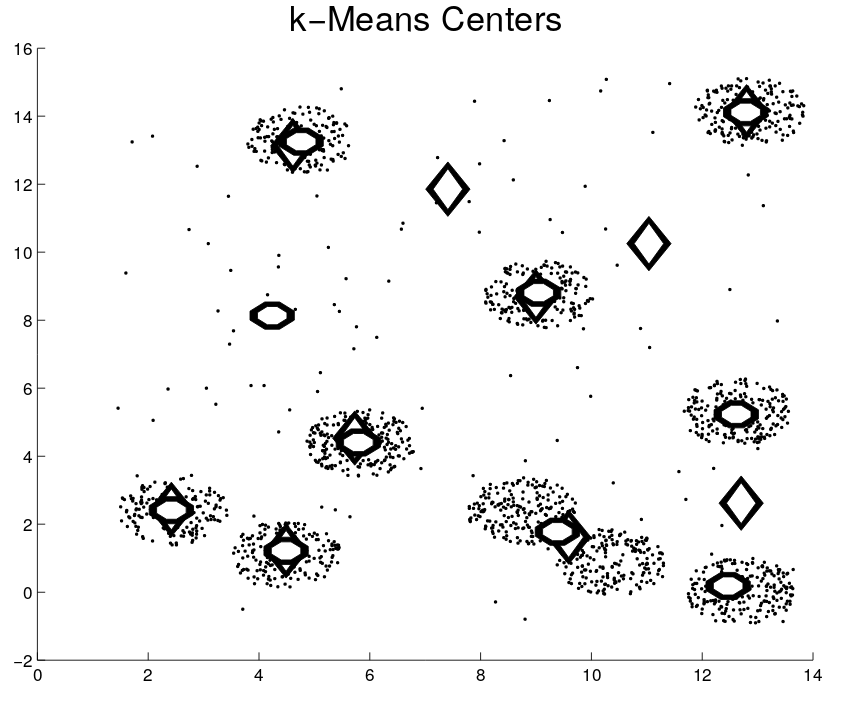
\includegraphics[width=\textwidth]{figures/k-means_clusters.png}      
        \end{center}
    \end{column}
    
  \end{columns}  
}

\frame
{
  \frametitle{LSEARCH vs k-means - results}
  % Include results on high dimensional data-sets? Talks about how LSEARCH finds better solution in the same time it takes k-means to find a solution
  
  \begin{columns}
  
    \begin{column}{0.4\textwidth}
    	  \begin{itemize}
    	  	\item[]{k-means:
    	  	  \begin{itemize}
    	  	    \item{Fails to distinguish two close centers}
    	  	    \item{Easily distracted by random noise}
    	  	    \item{Comparatively high variance in SSQ}
    	  	  \end{itemize}
    	  	}
    	  	\item[]{LSEARCH:
    	  	  \begin{itemize}
    	  	    \item{Low variance in SSQ across all data-sets, consistently close to optimal}
    	  	  \end{itemize}
    	  	}
    	  \end{itemize}
    	  
    \end{column}
    
    \begin{column}{0.6\textwidth}
        \begin{center}
         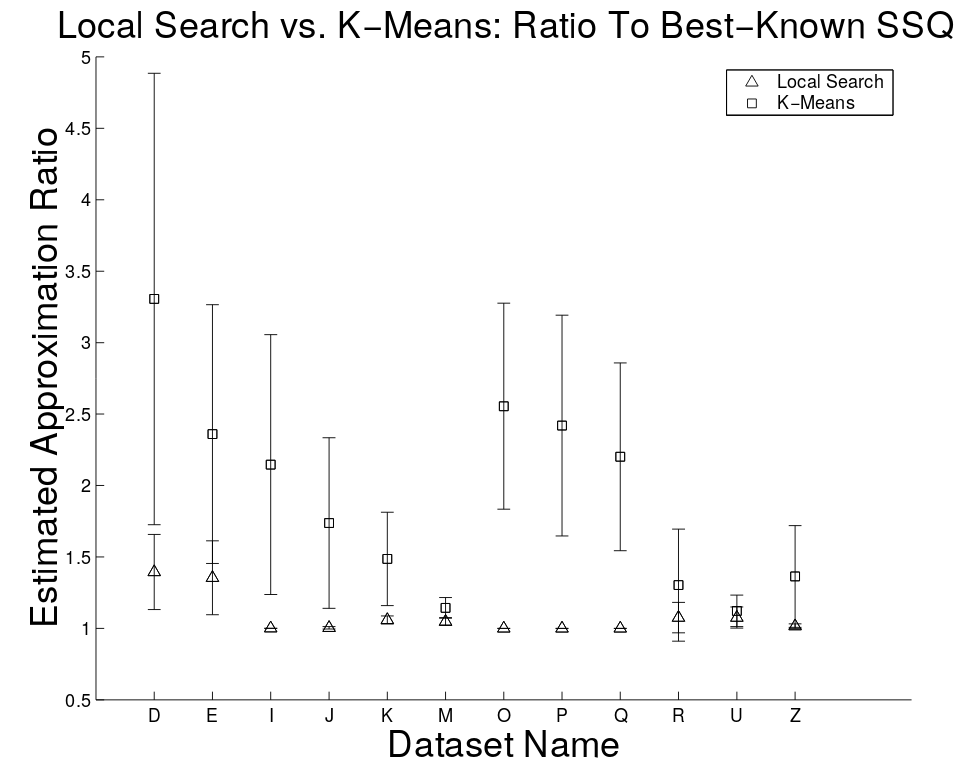
\includegraphics[width=\textwidth]{figures/LSEARCH_vs_k-means.png}      
        \end{center}
    \end{column}
    
  \end{columns}  
}


\frame
{
  \frametitle{STREAM vs BIRCH}
%  BIRCH uses a CF-tree to compress a large set of data. The leaves of the CF-tree contain sufficient statistics for a subset of points. A clustering algorithm then clusters the leaf entries. Both STREAM and BIRCH repeatedly pre-cluster the data. 

  \begin{itemize}
	\item{Generated data-set with $50,000$ $40$-dimensional points, arranged in clusters with overlaid random noise.}
	\item{Clustered the data-set 10 times using each of:
	  \begin{itemize}
	  	\item{BIRCH with k-means}
	  	\item{BIRCH with LSEARCH}
	  	\item{STREAM with k-means}
	  	\item{STREAM with LSEARCH}
	  \end{itemize}	   
	}
	\item{SSQ and CPU run-time were used as comparison factors}
  \end{itemize}

}

\frame
{
  \frametitle{STREAM vs BIRCH - results}
  
  \begin{columns}
  
    \begin{column}{0.5\textwidth}
    	   \begin{center}
         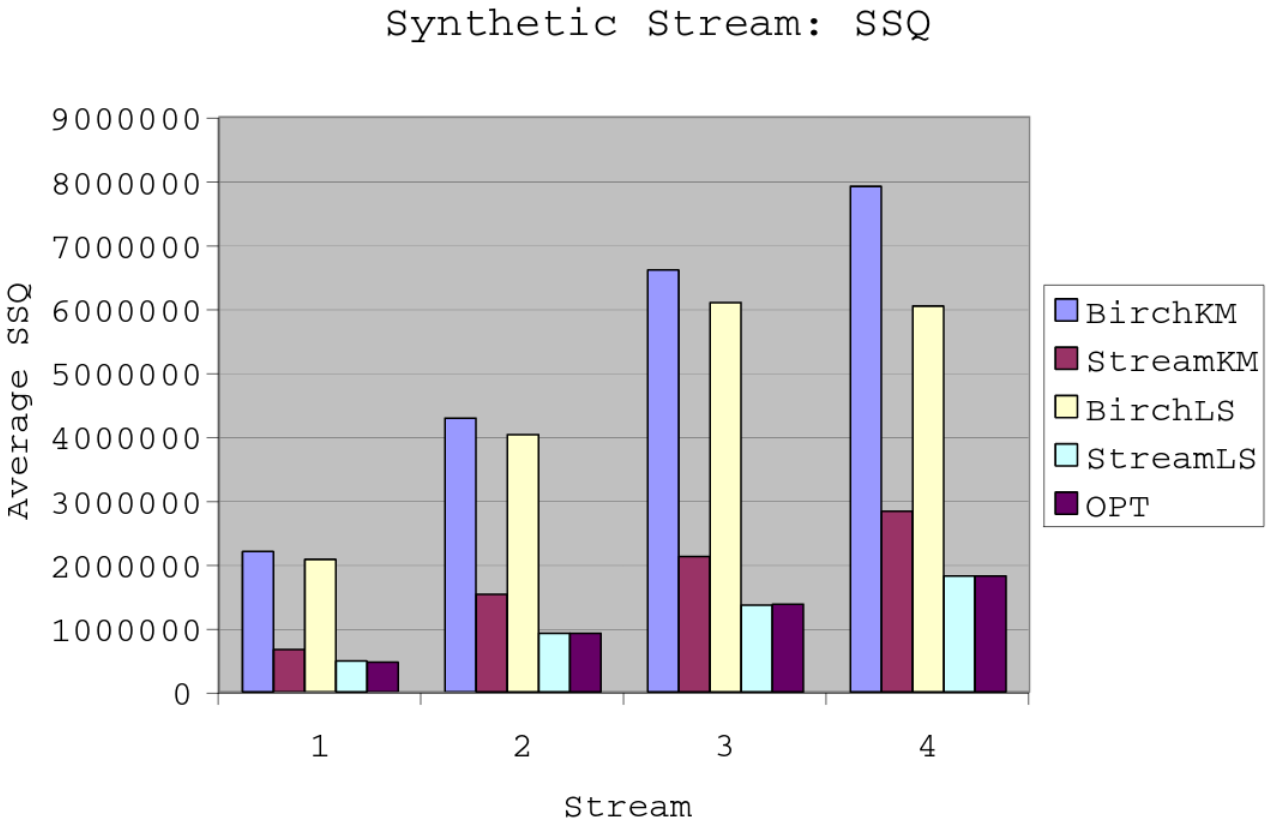
\includegraphics[width=\textwidth]{figures/BIRCH_STREAM_SSQ.png}      
       \end{center}
    	  
    \end{column}
    
    \begin{column}{0.5\textwidth}
        \begin{center}
         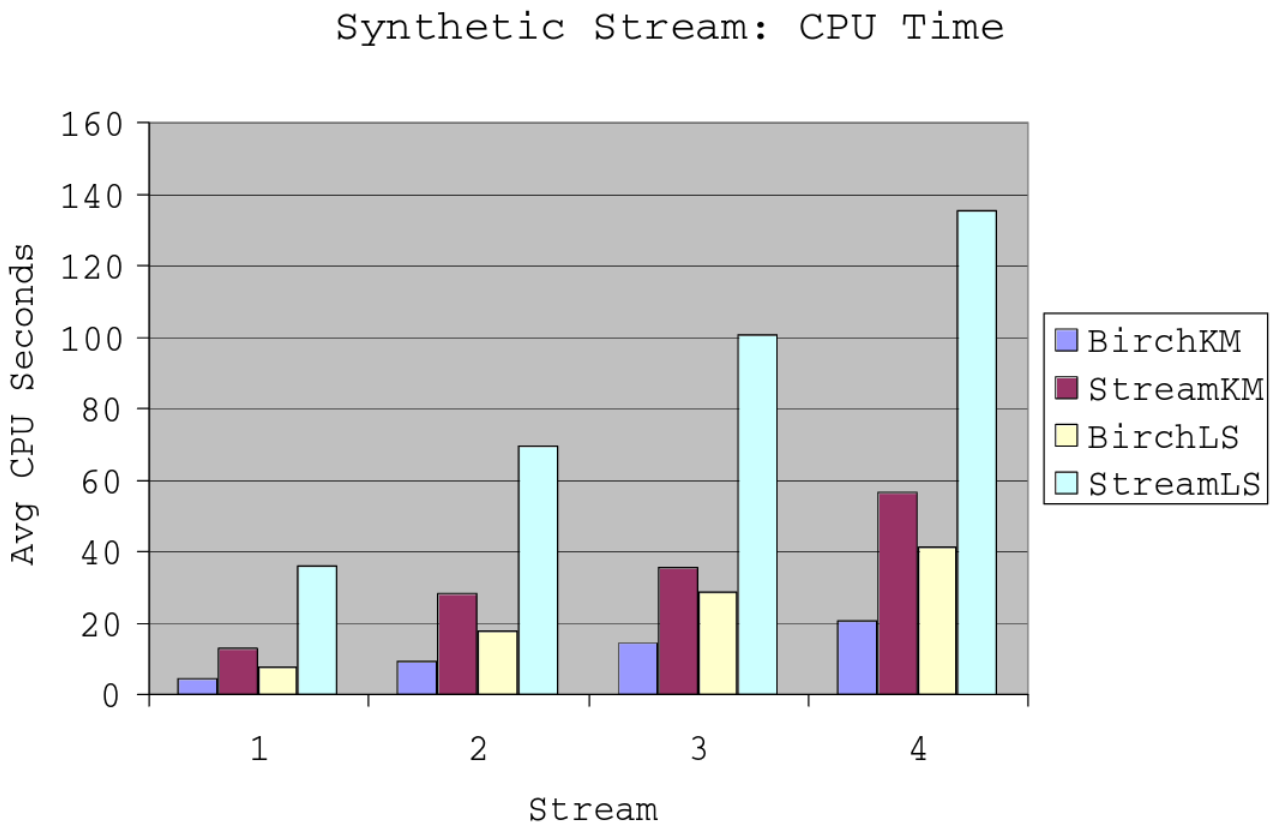
\includegraphics[width=\textwidth]{figures/BIRCH_STREAM_CPU.png}      
        \end{center}
    \end{column}
  \end{columns}  
  
  \bigskip
  STREAM with k-means gives the best balance between low CPU time and low SSQ. STREAM with LSEARCH finds the closest solution to optimal, but with the highest CPU time. BIRCH with k-means gives the best CPU time but the worst SSQ.
}



\frame[t]{
  \frametitle{References}

  O'Callaghan, L., Mishra, N., Meyerson, A., Guha, S. \& Motwani,
  R. (2002). \textit{Streaming-data algorithms for high-quality
    clustering.} In proceedings of the 18th International Conference
  on Data Engineering. Available from:
  http://ieeexplore.ieee.org/document/994785/.  }
  
\end{document}
